%===================================== CHAP 4 =================================

\chapter{Implementation}
\section{Mechanical}

The brackets for the Moteus boards were 3D-printed in PETG in two parts and assembled to the motors using M2.5 screws,
see \autoref{fig:bracket-printed}.

\begin{figure}[H]
  \centering
  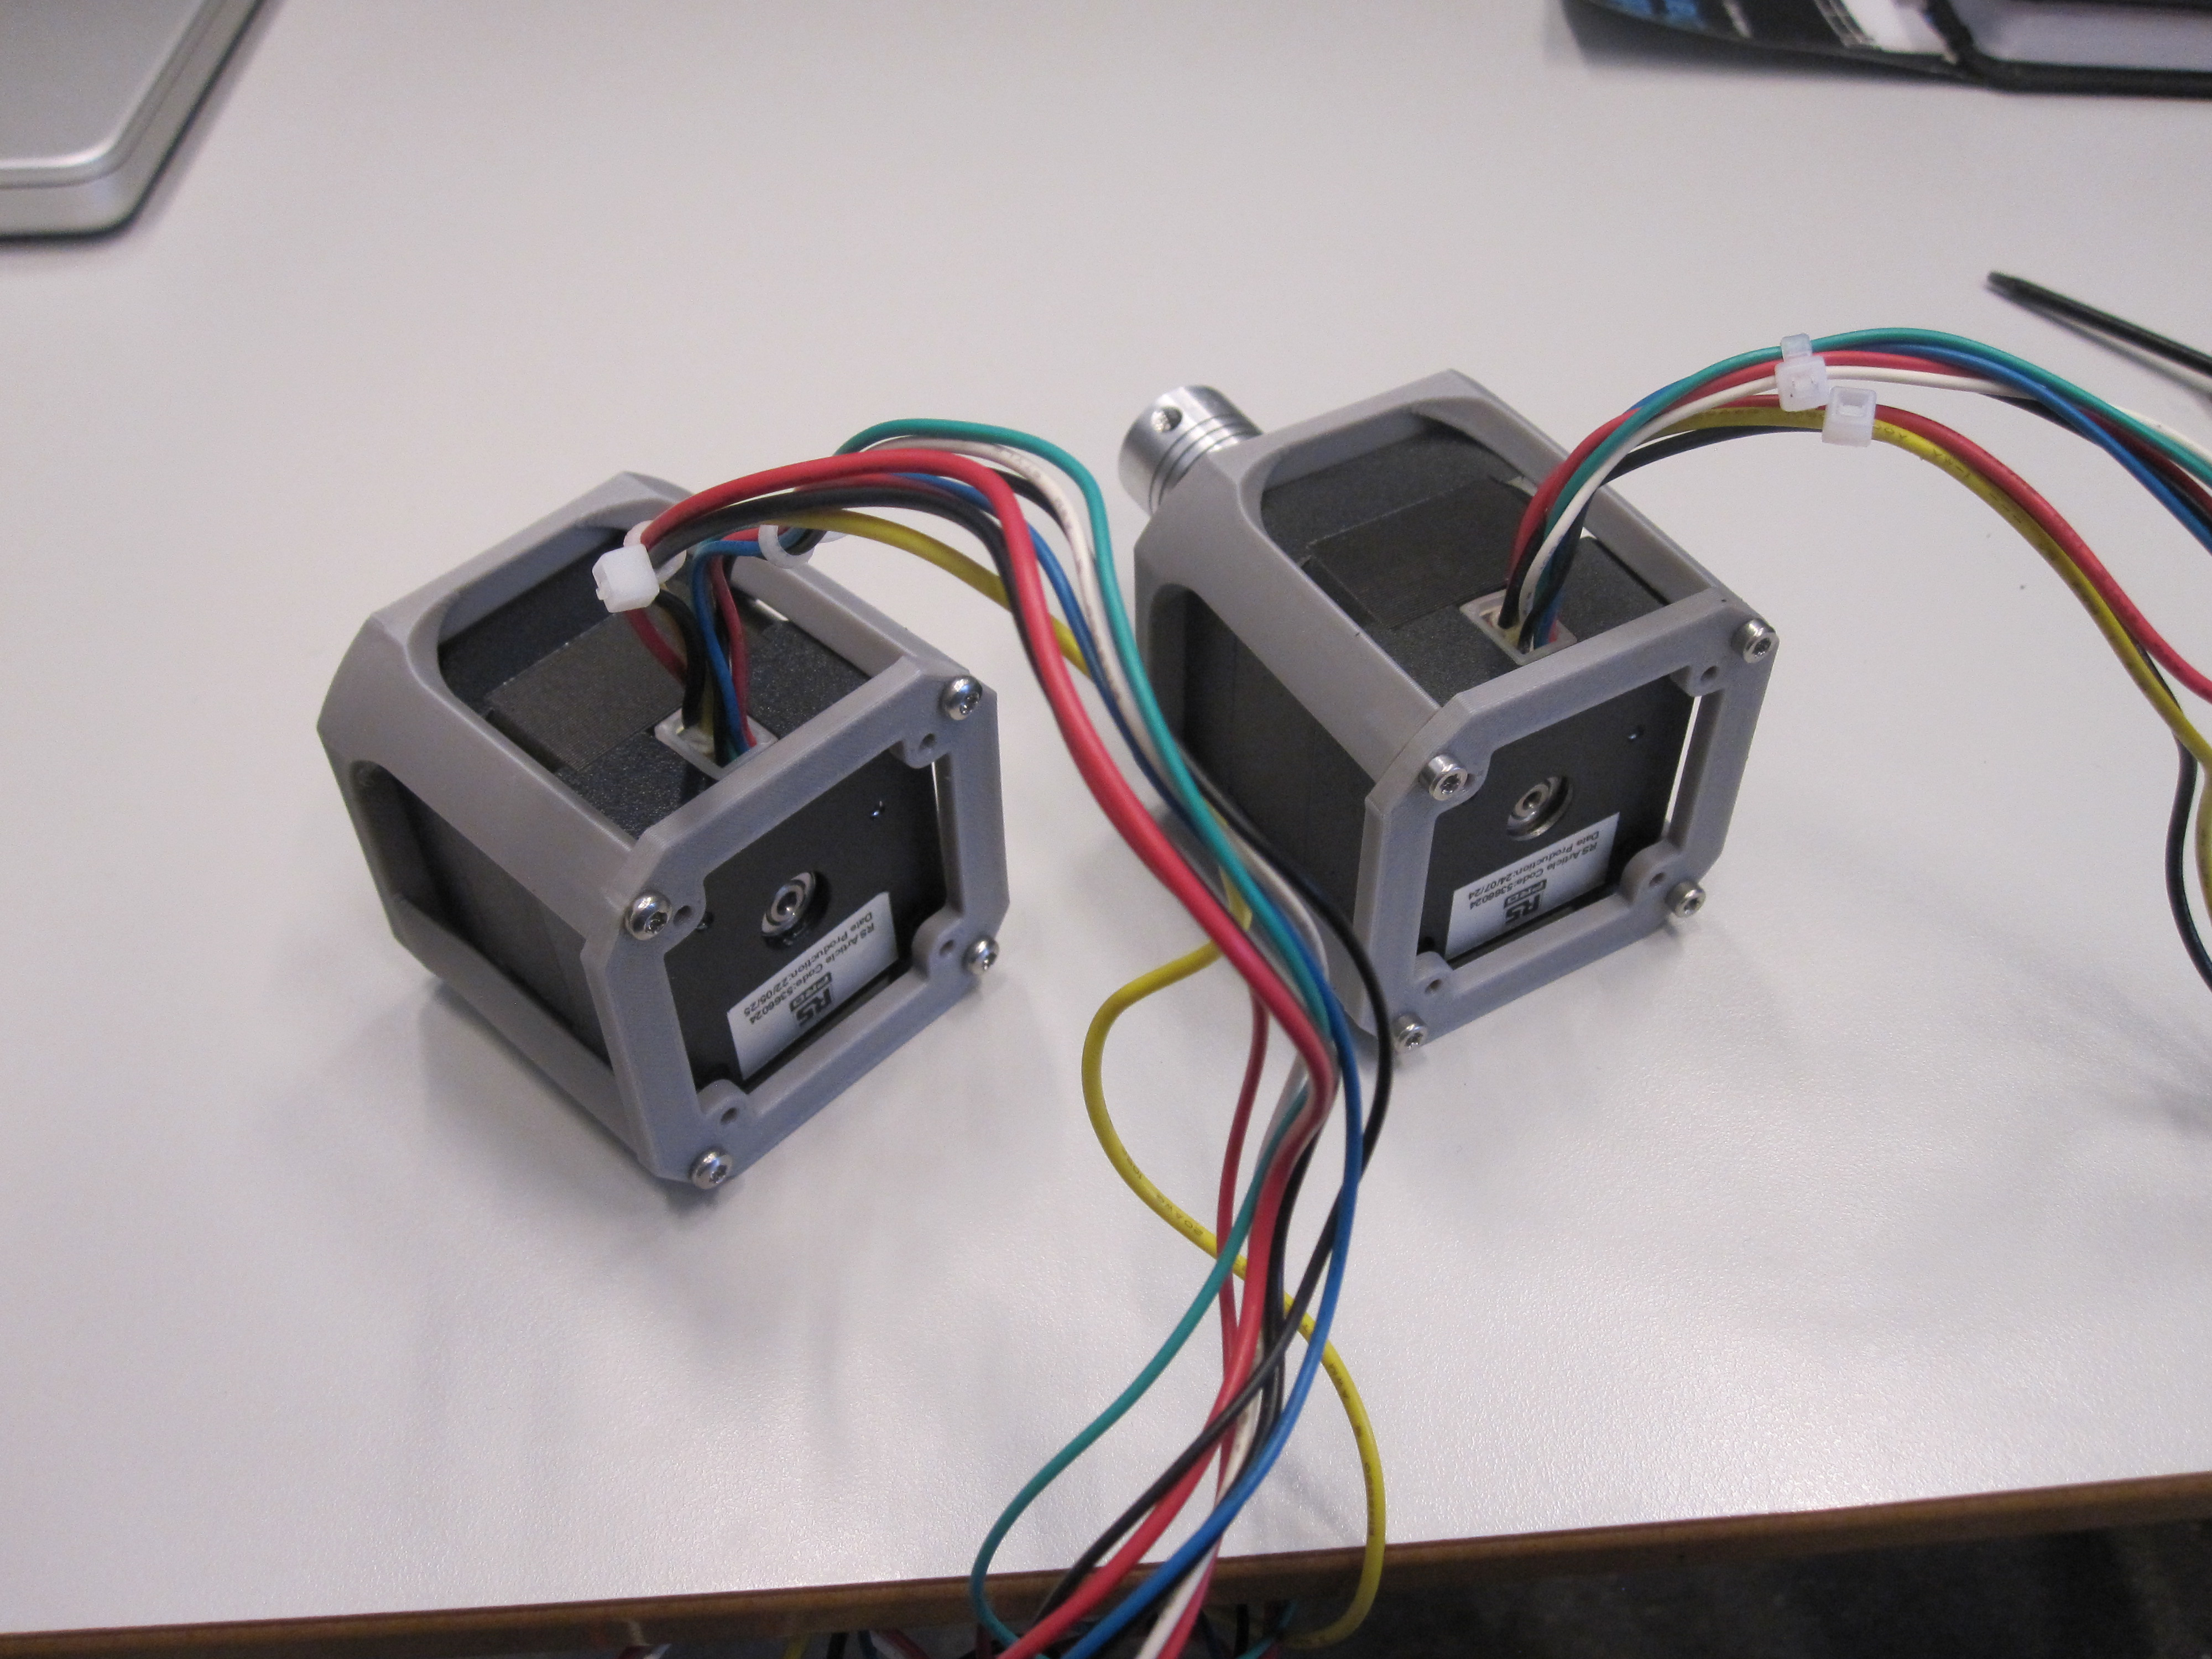
\includegraphics[width=0.4\textwidth]{fig/motor-bracket-back}\hfill
  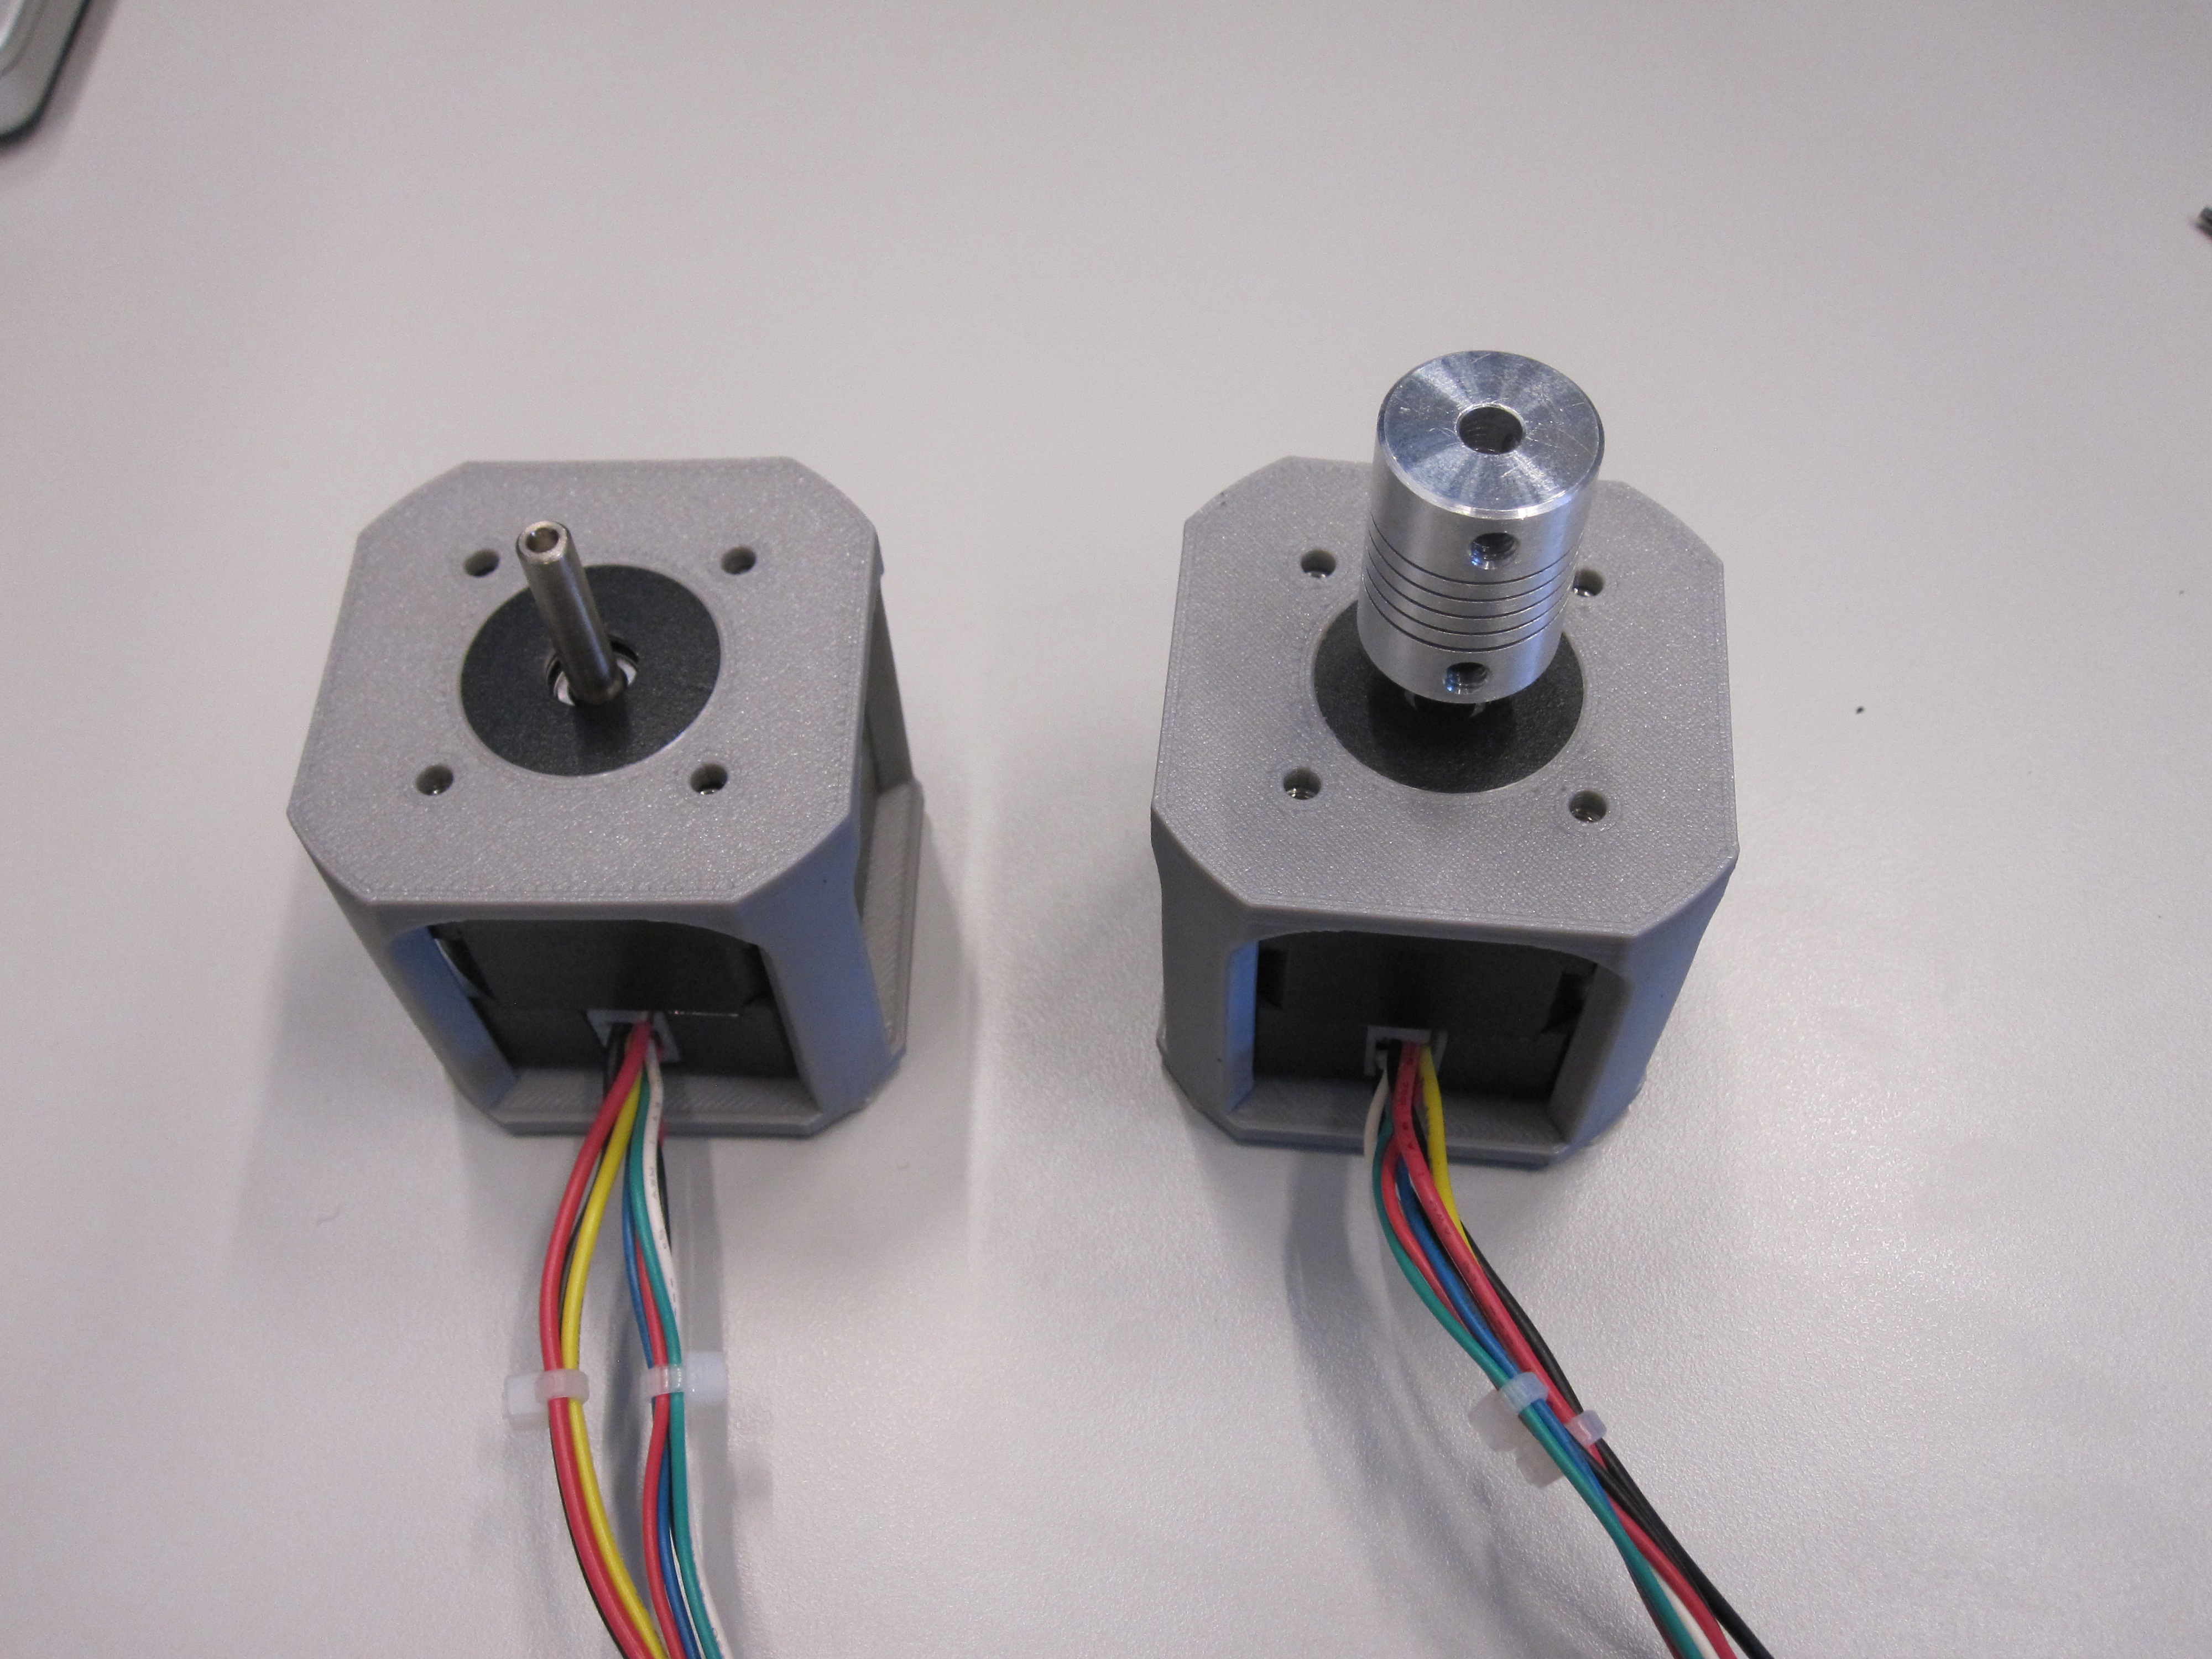
\includegraphics[width=0.4\textwidth]{fig/motor-bracket-front}\hfill
  \caption{}
  \label{fig:bracket-printed}
\end{figure}

The bearing seat was 3D-printed in PETG and the bearing was pressed into the seat, see \autoref{fig:bearing-seat-printed}.

\begin{figure}[H]
  \centering
  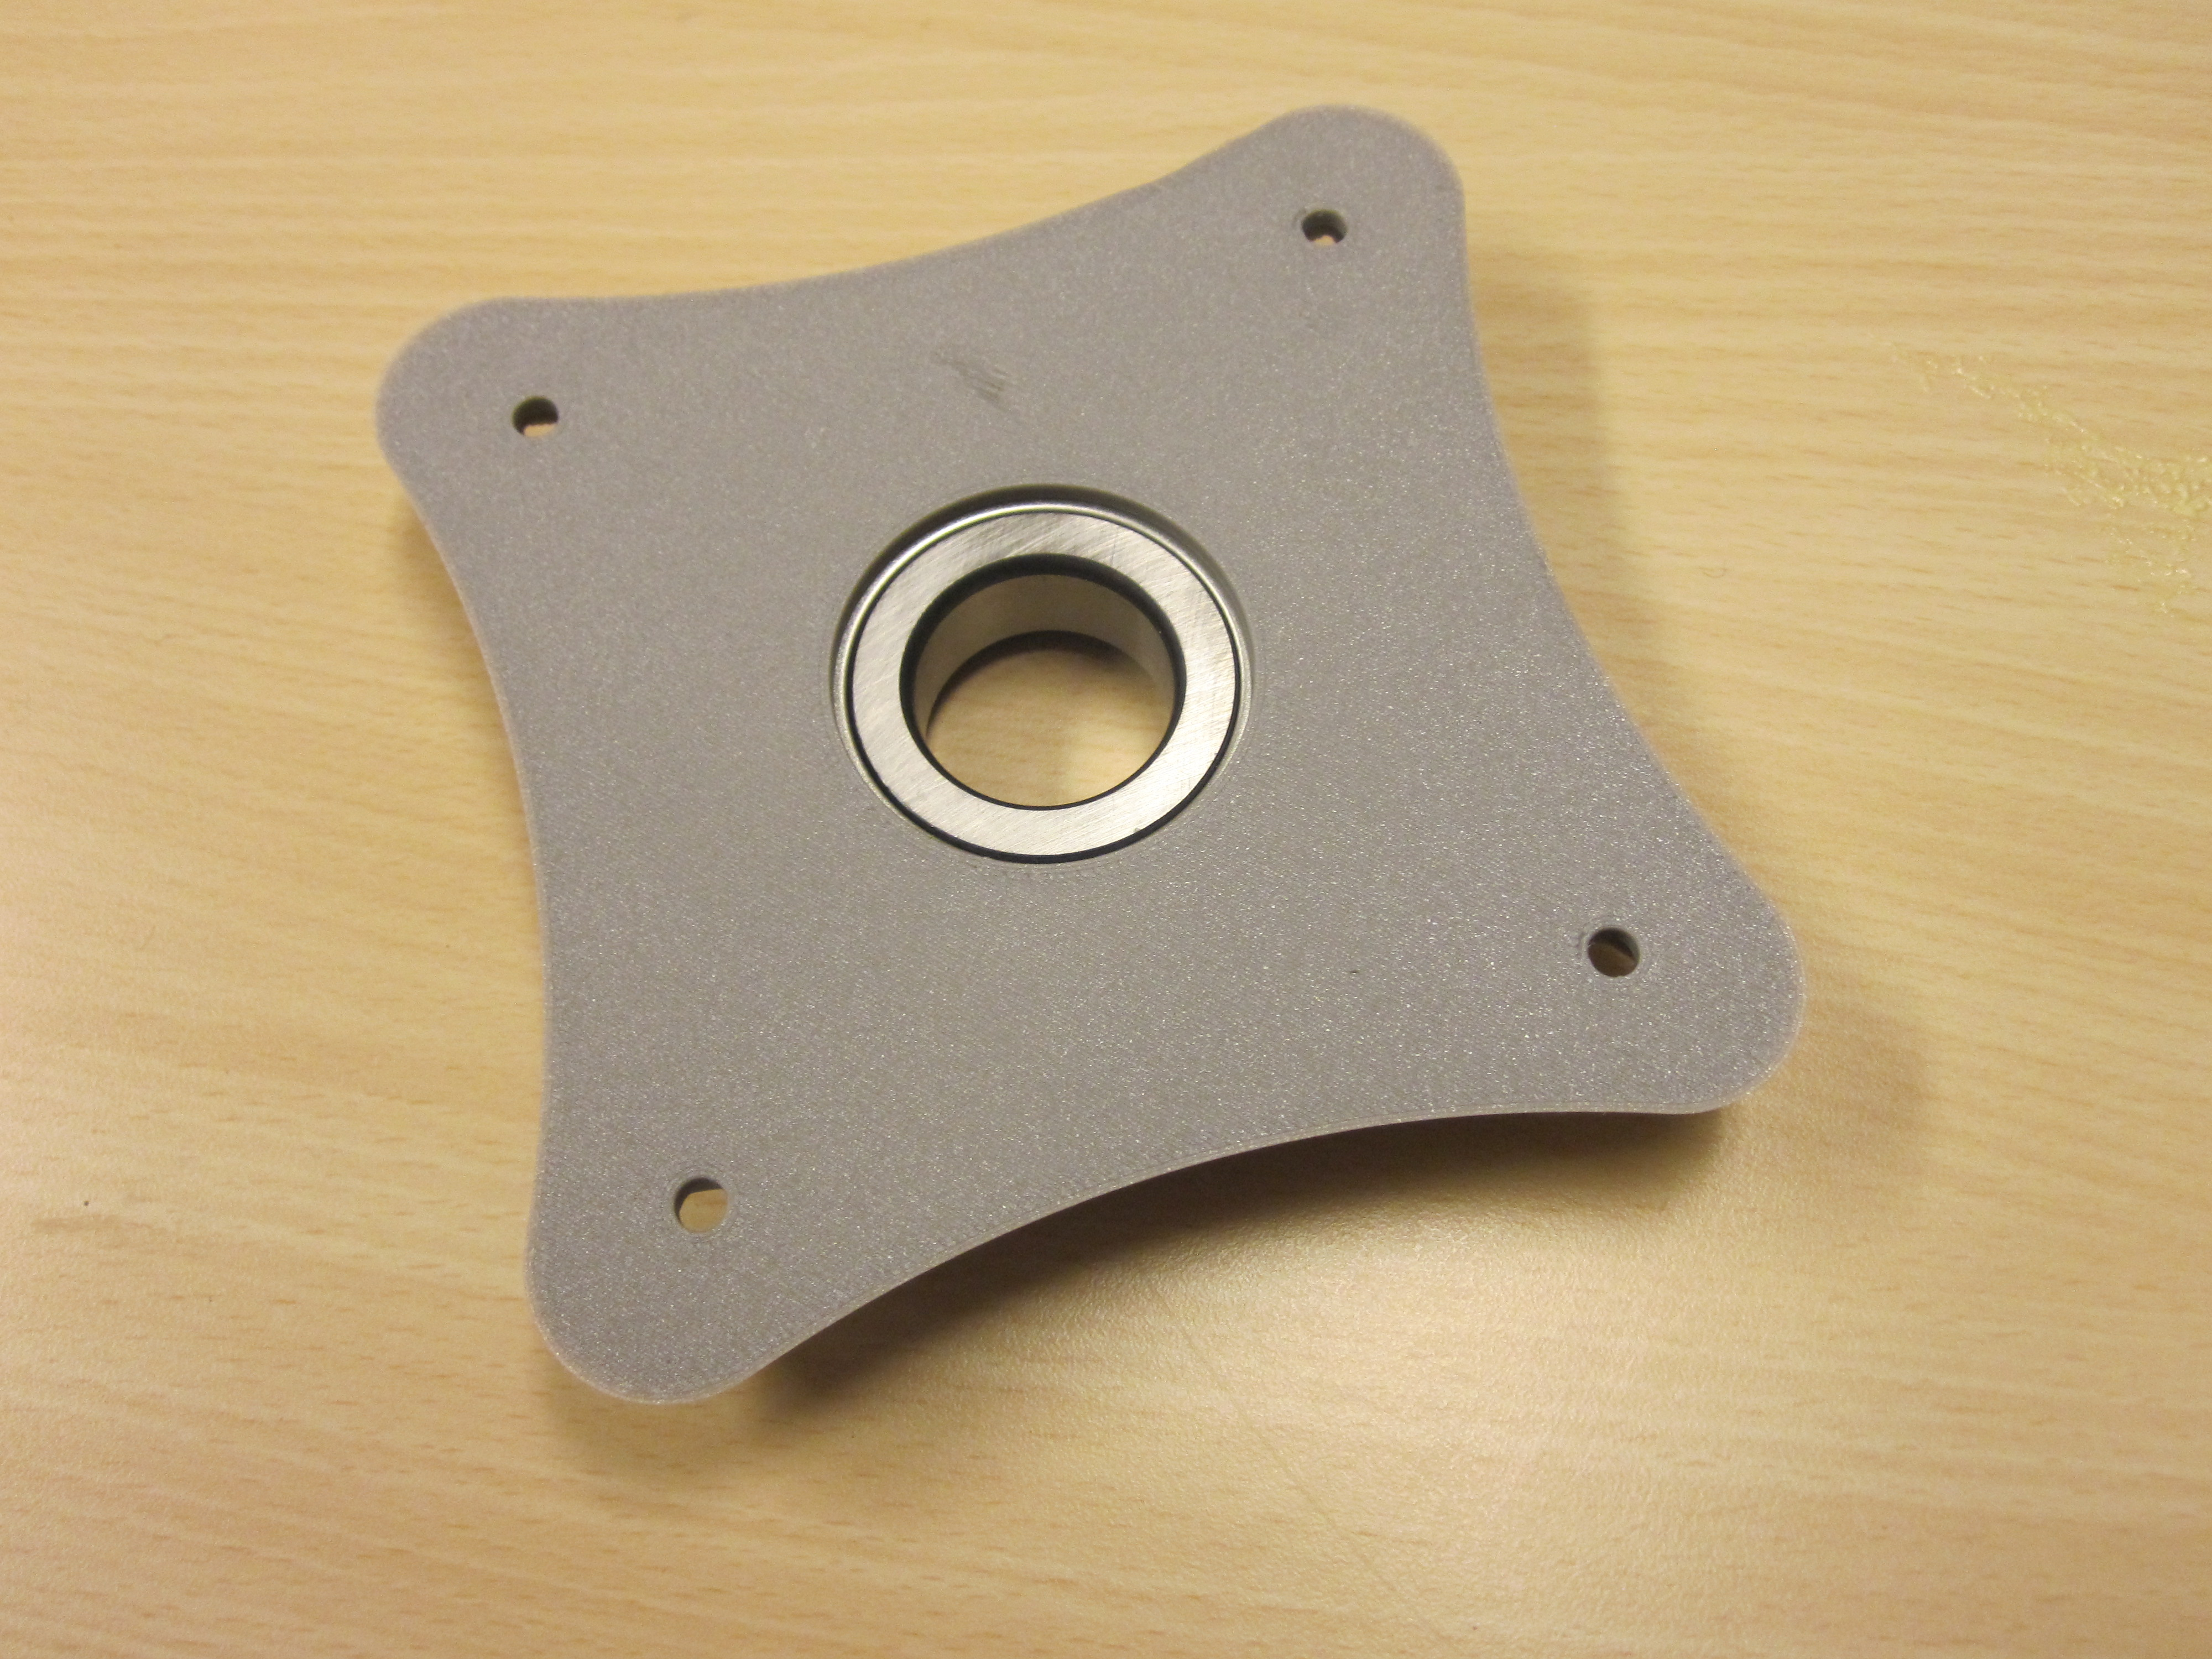
\includegraphics[width=0.4\textwidth]{fig/bearing-seat-back}\hfill
  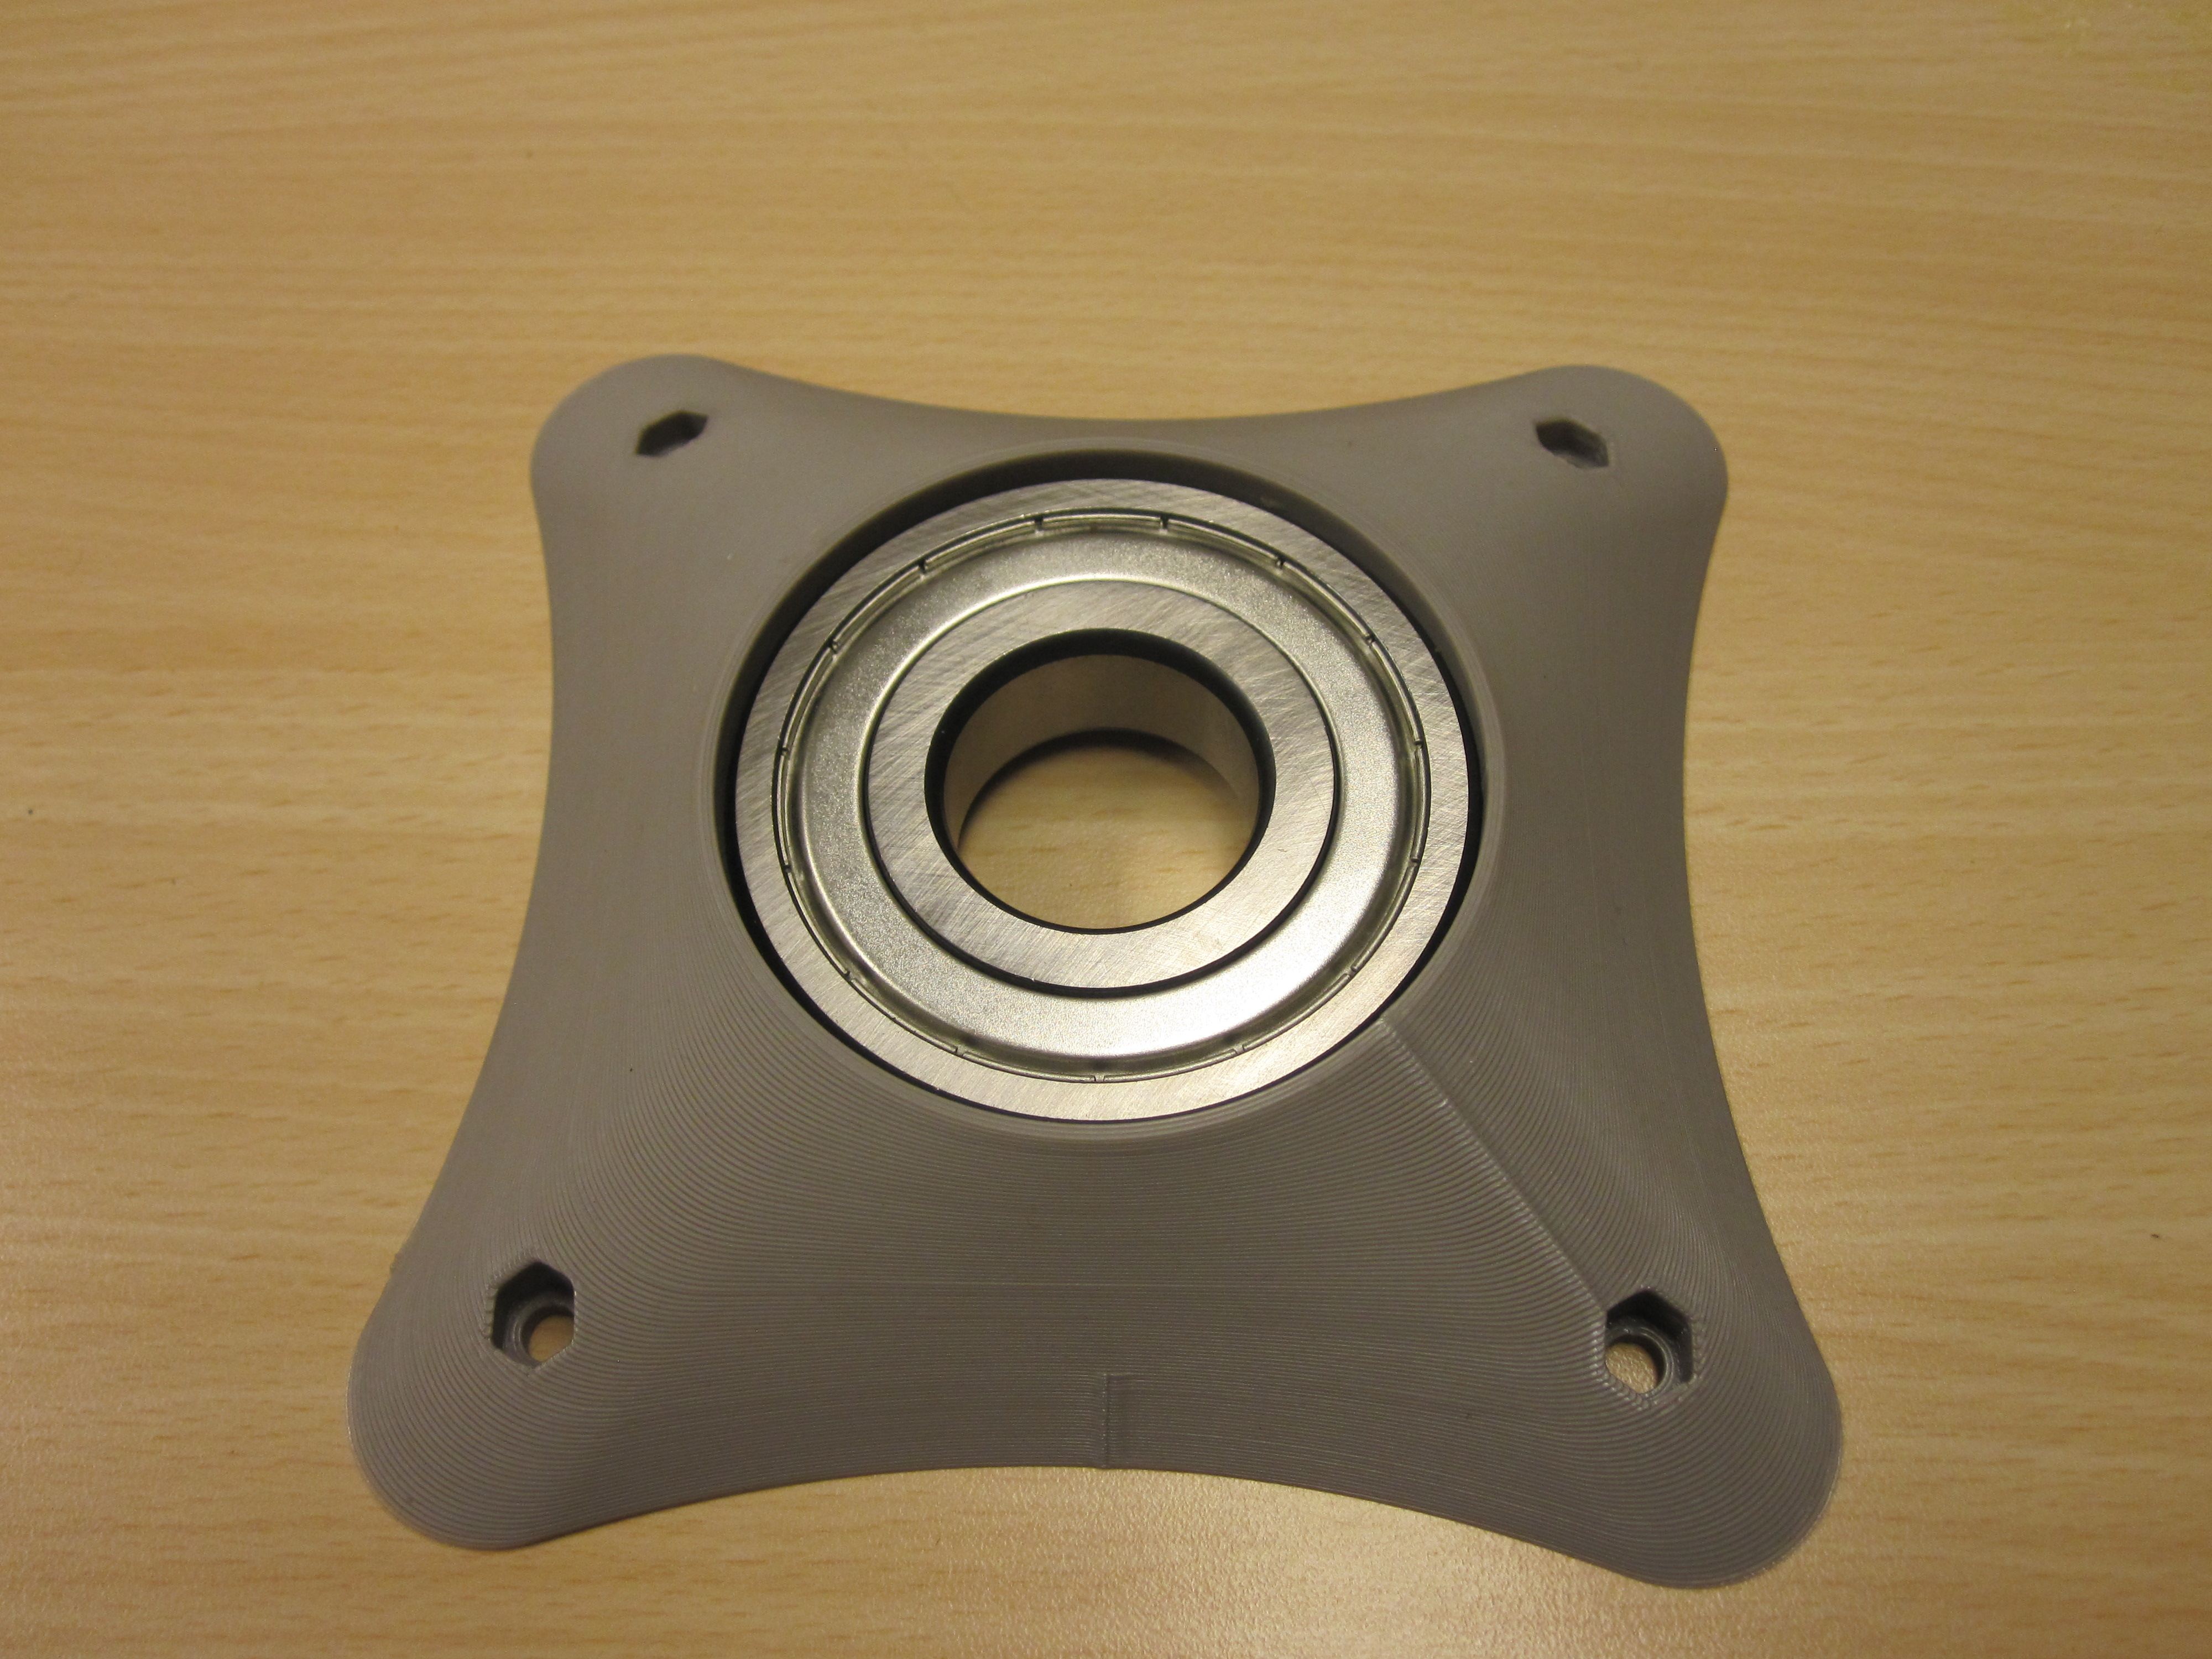
\includegraphics[width=0.4\textwidth]{fig/bearing-seat-front}\hfill
  \caption{}
  \label{fig:bearing-seat-printed}
\end{figure}

A diametrically magentized magnet was glued to the back the rotor using a drop of super glue, see 
\autoref{fig:glued-magnet}

\begin{figure}[H]
  \centering
  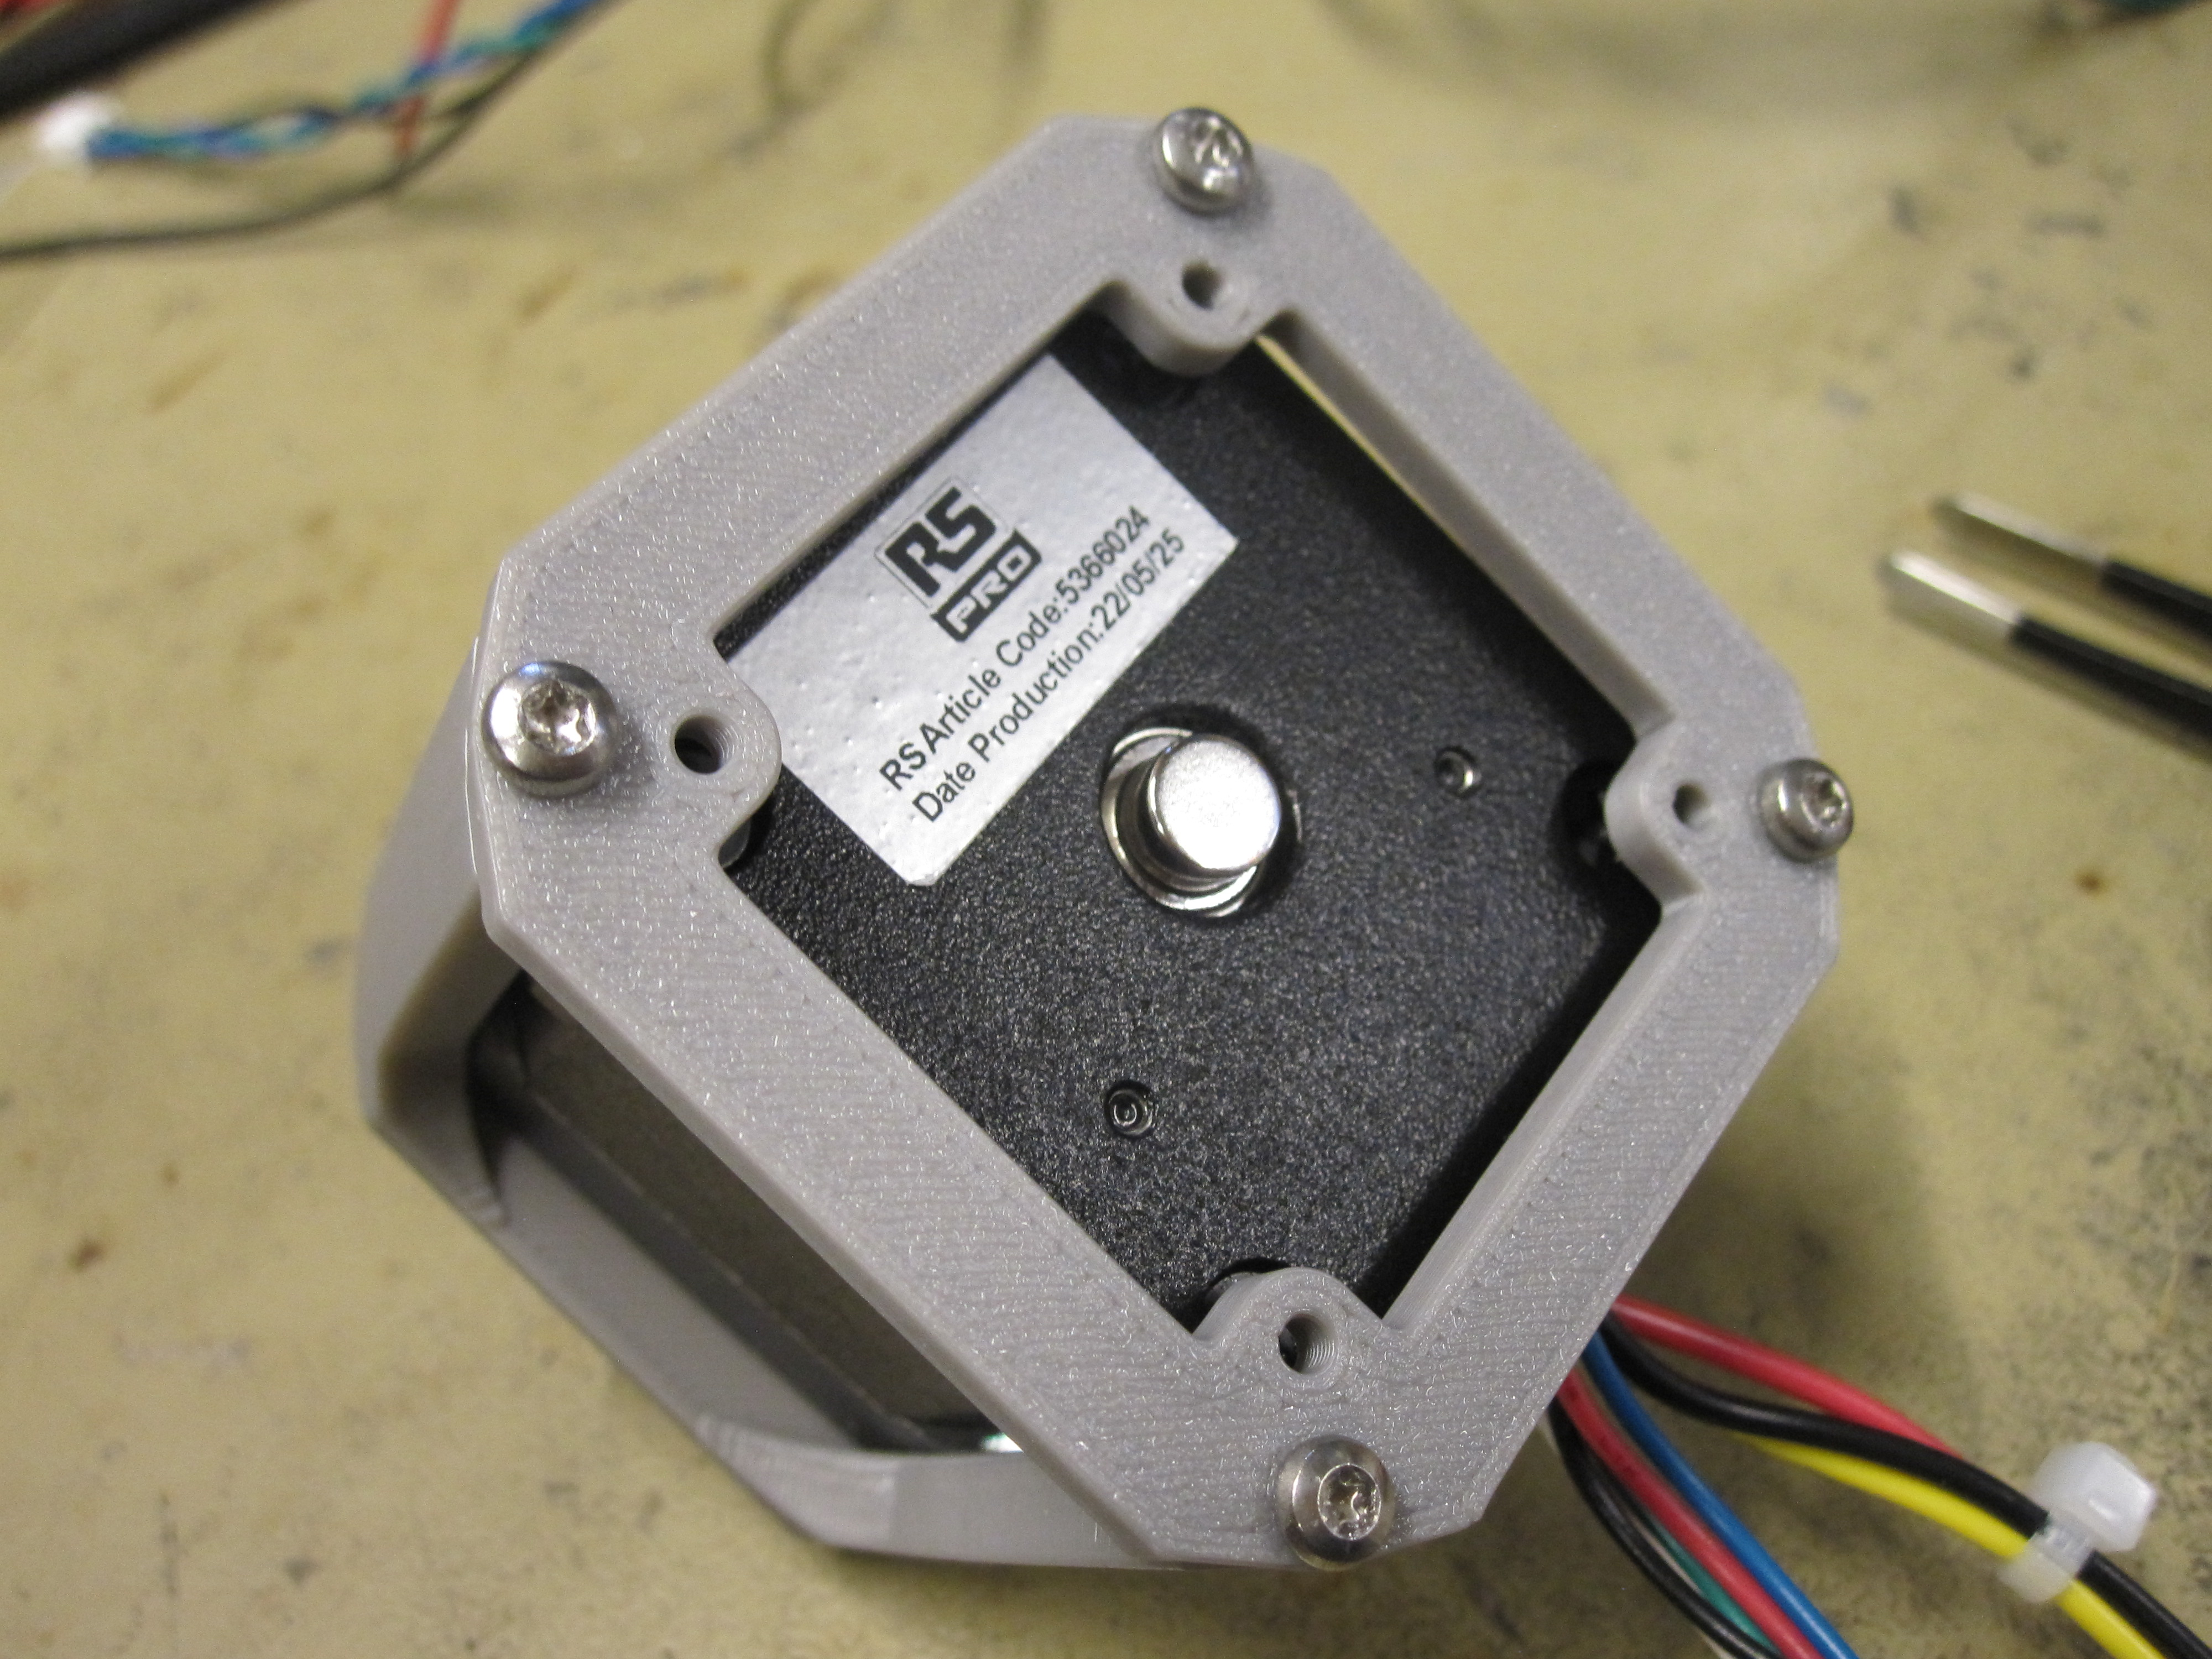
\includegraphics[width=0.7\textwidth]{fig/implementation/glued-magnet.JPG}\hfill
  \caption{Motor with magned glued to the back of the rotor.}
  \label{fig:glued-magnet}
\end{figure}


\section{Hardware}
Power cables for the Moteus motor divers were constructed by soldering a XT30 connector on one end, following the instructions from Moteus
(link).
A fuse holder was joined to the cable with a butt splice and the other end of the cable was termintated with 
bootlace ferrules for secure connection to the terminals of the Power supply unit. The cable is shown in \autoref{fig:powercable}.


\begin{figure}[H]
  \centering
  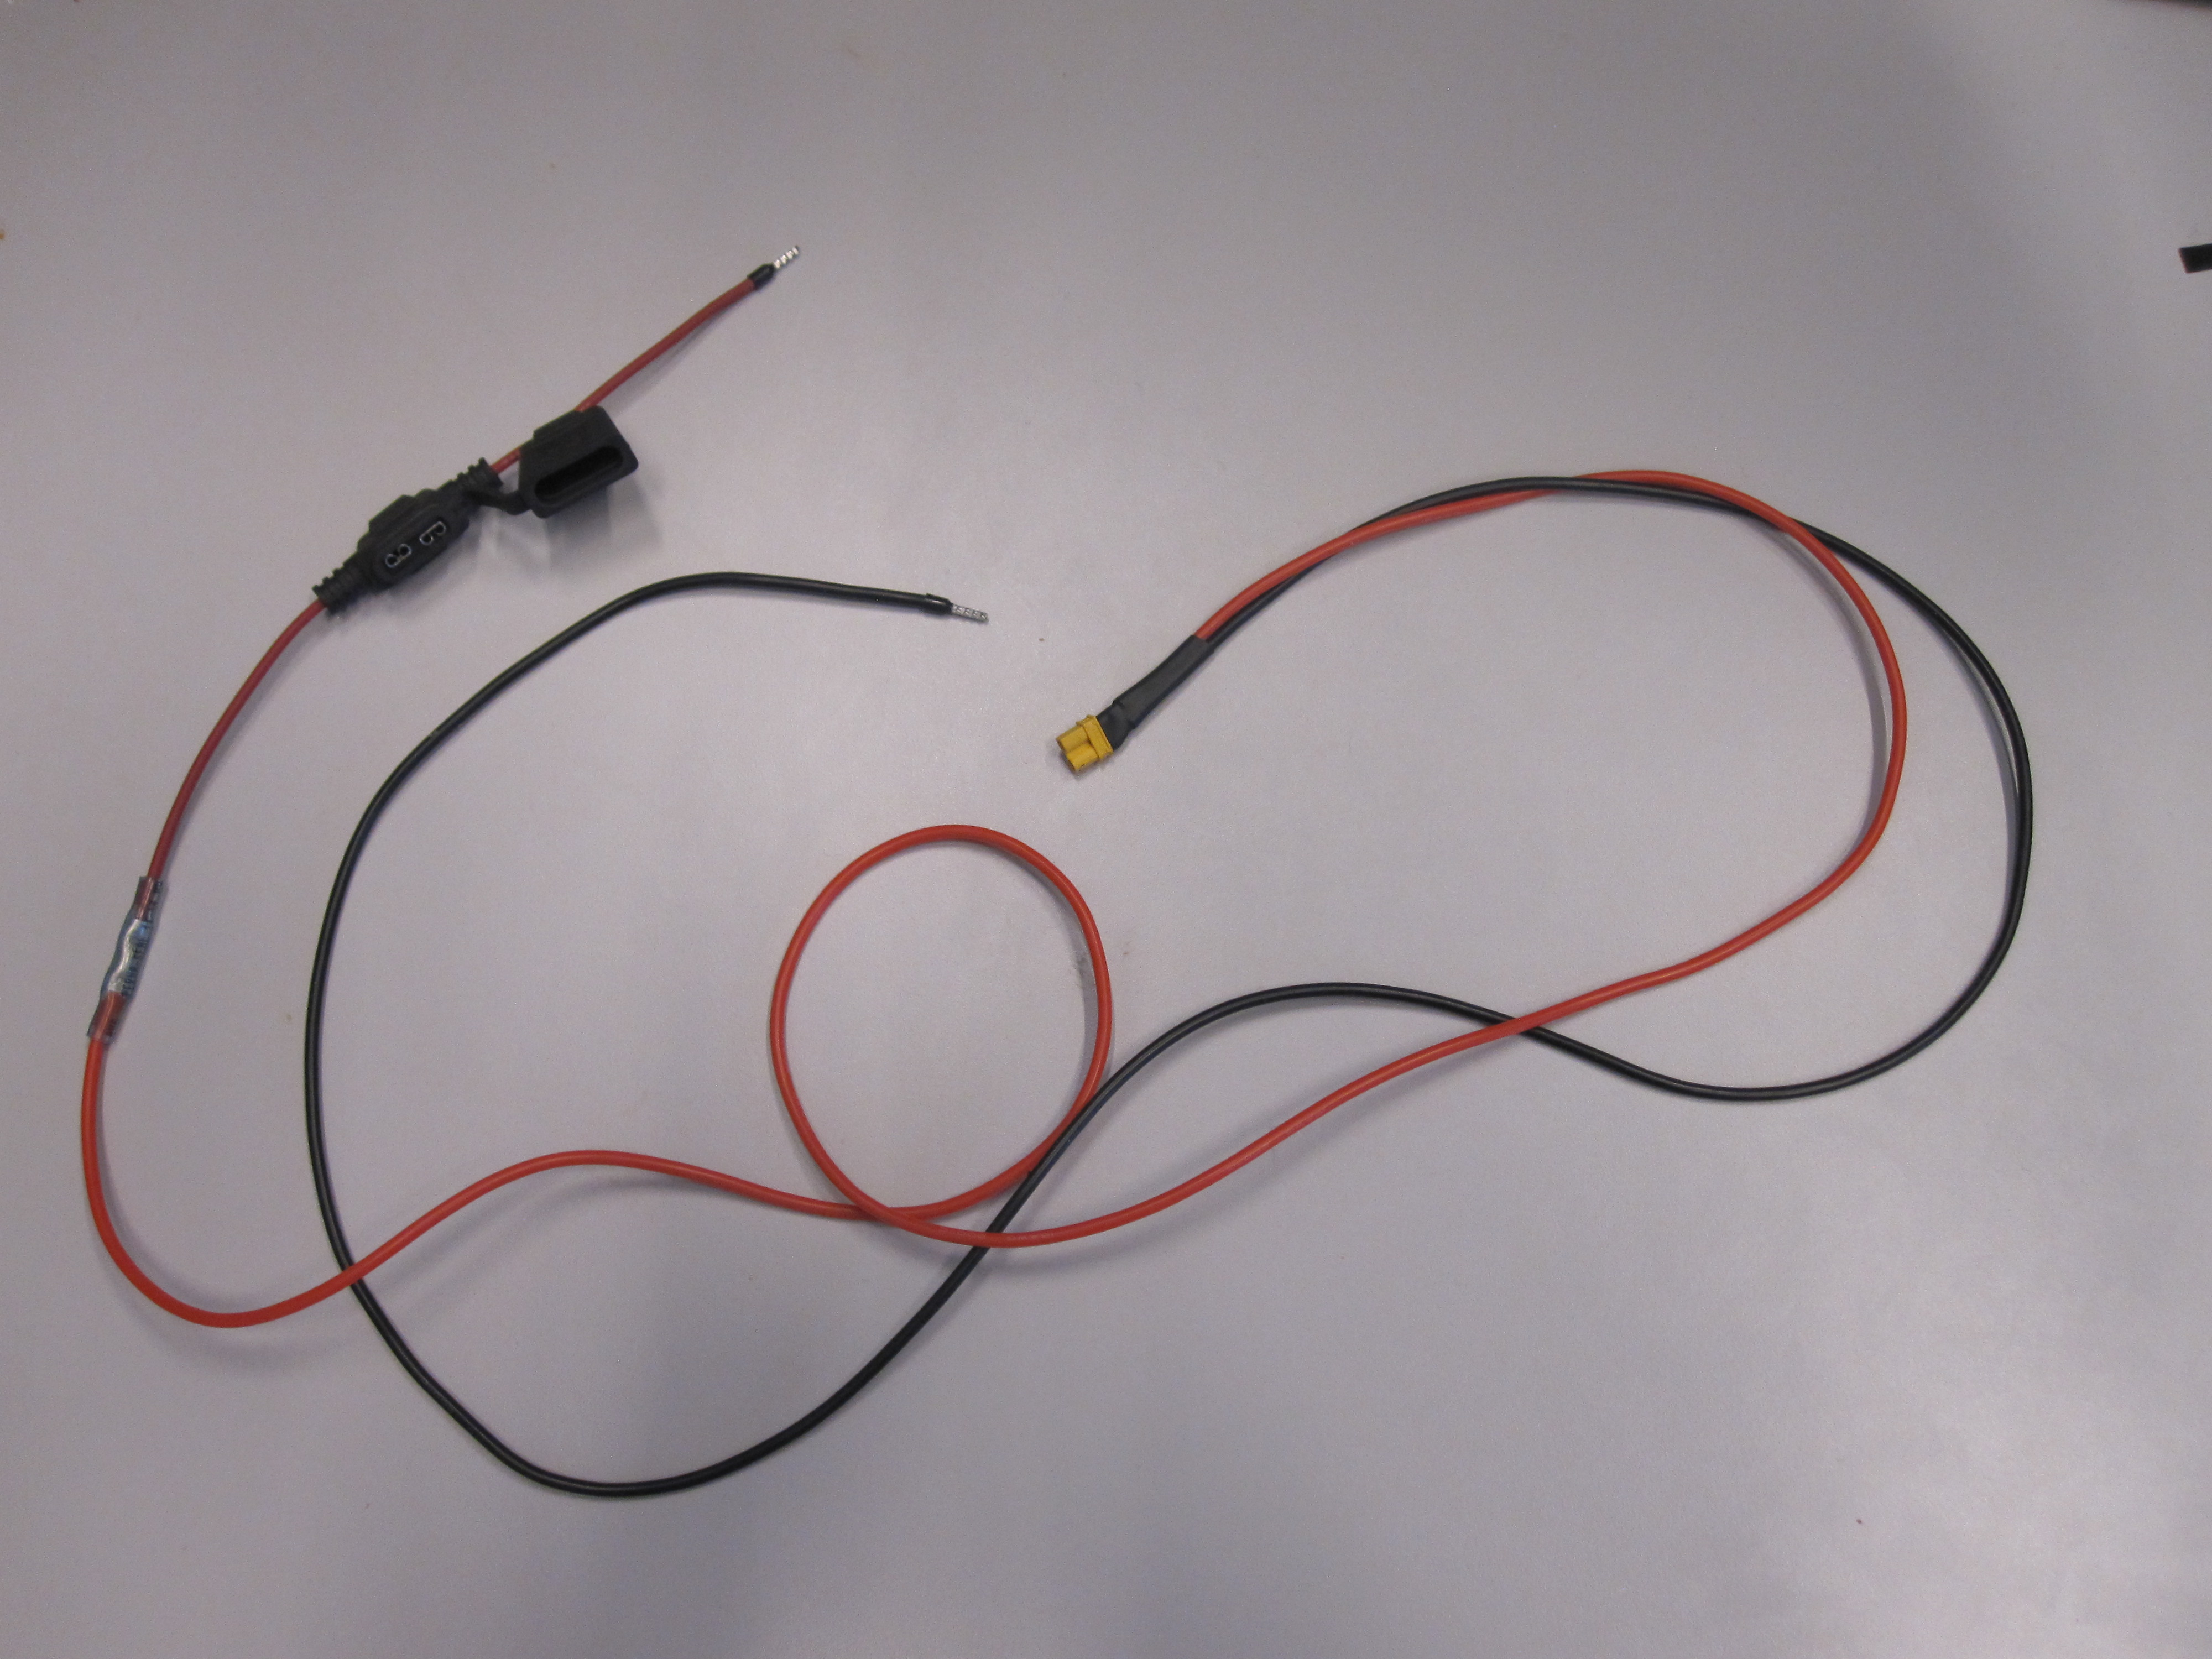
\includegraphics[width=0.7\textwidth]{fig/implementation/power-cord.JPG}\hfill
  \caption{}
  \label{fig:powercable}
\end{figure}


Phase wires were soldered to the Moteus boards, see \autoref{fig:soldered-moteus}

\begin{figure}[H]
  \centering
  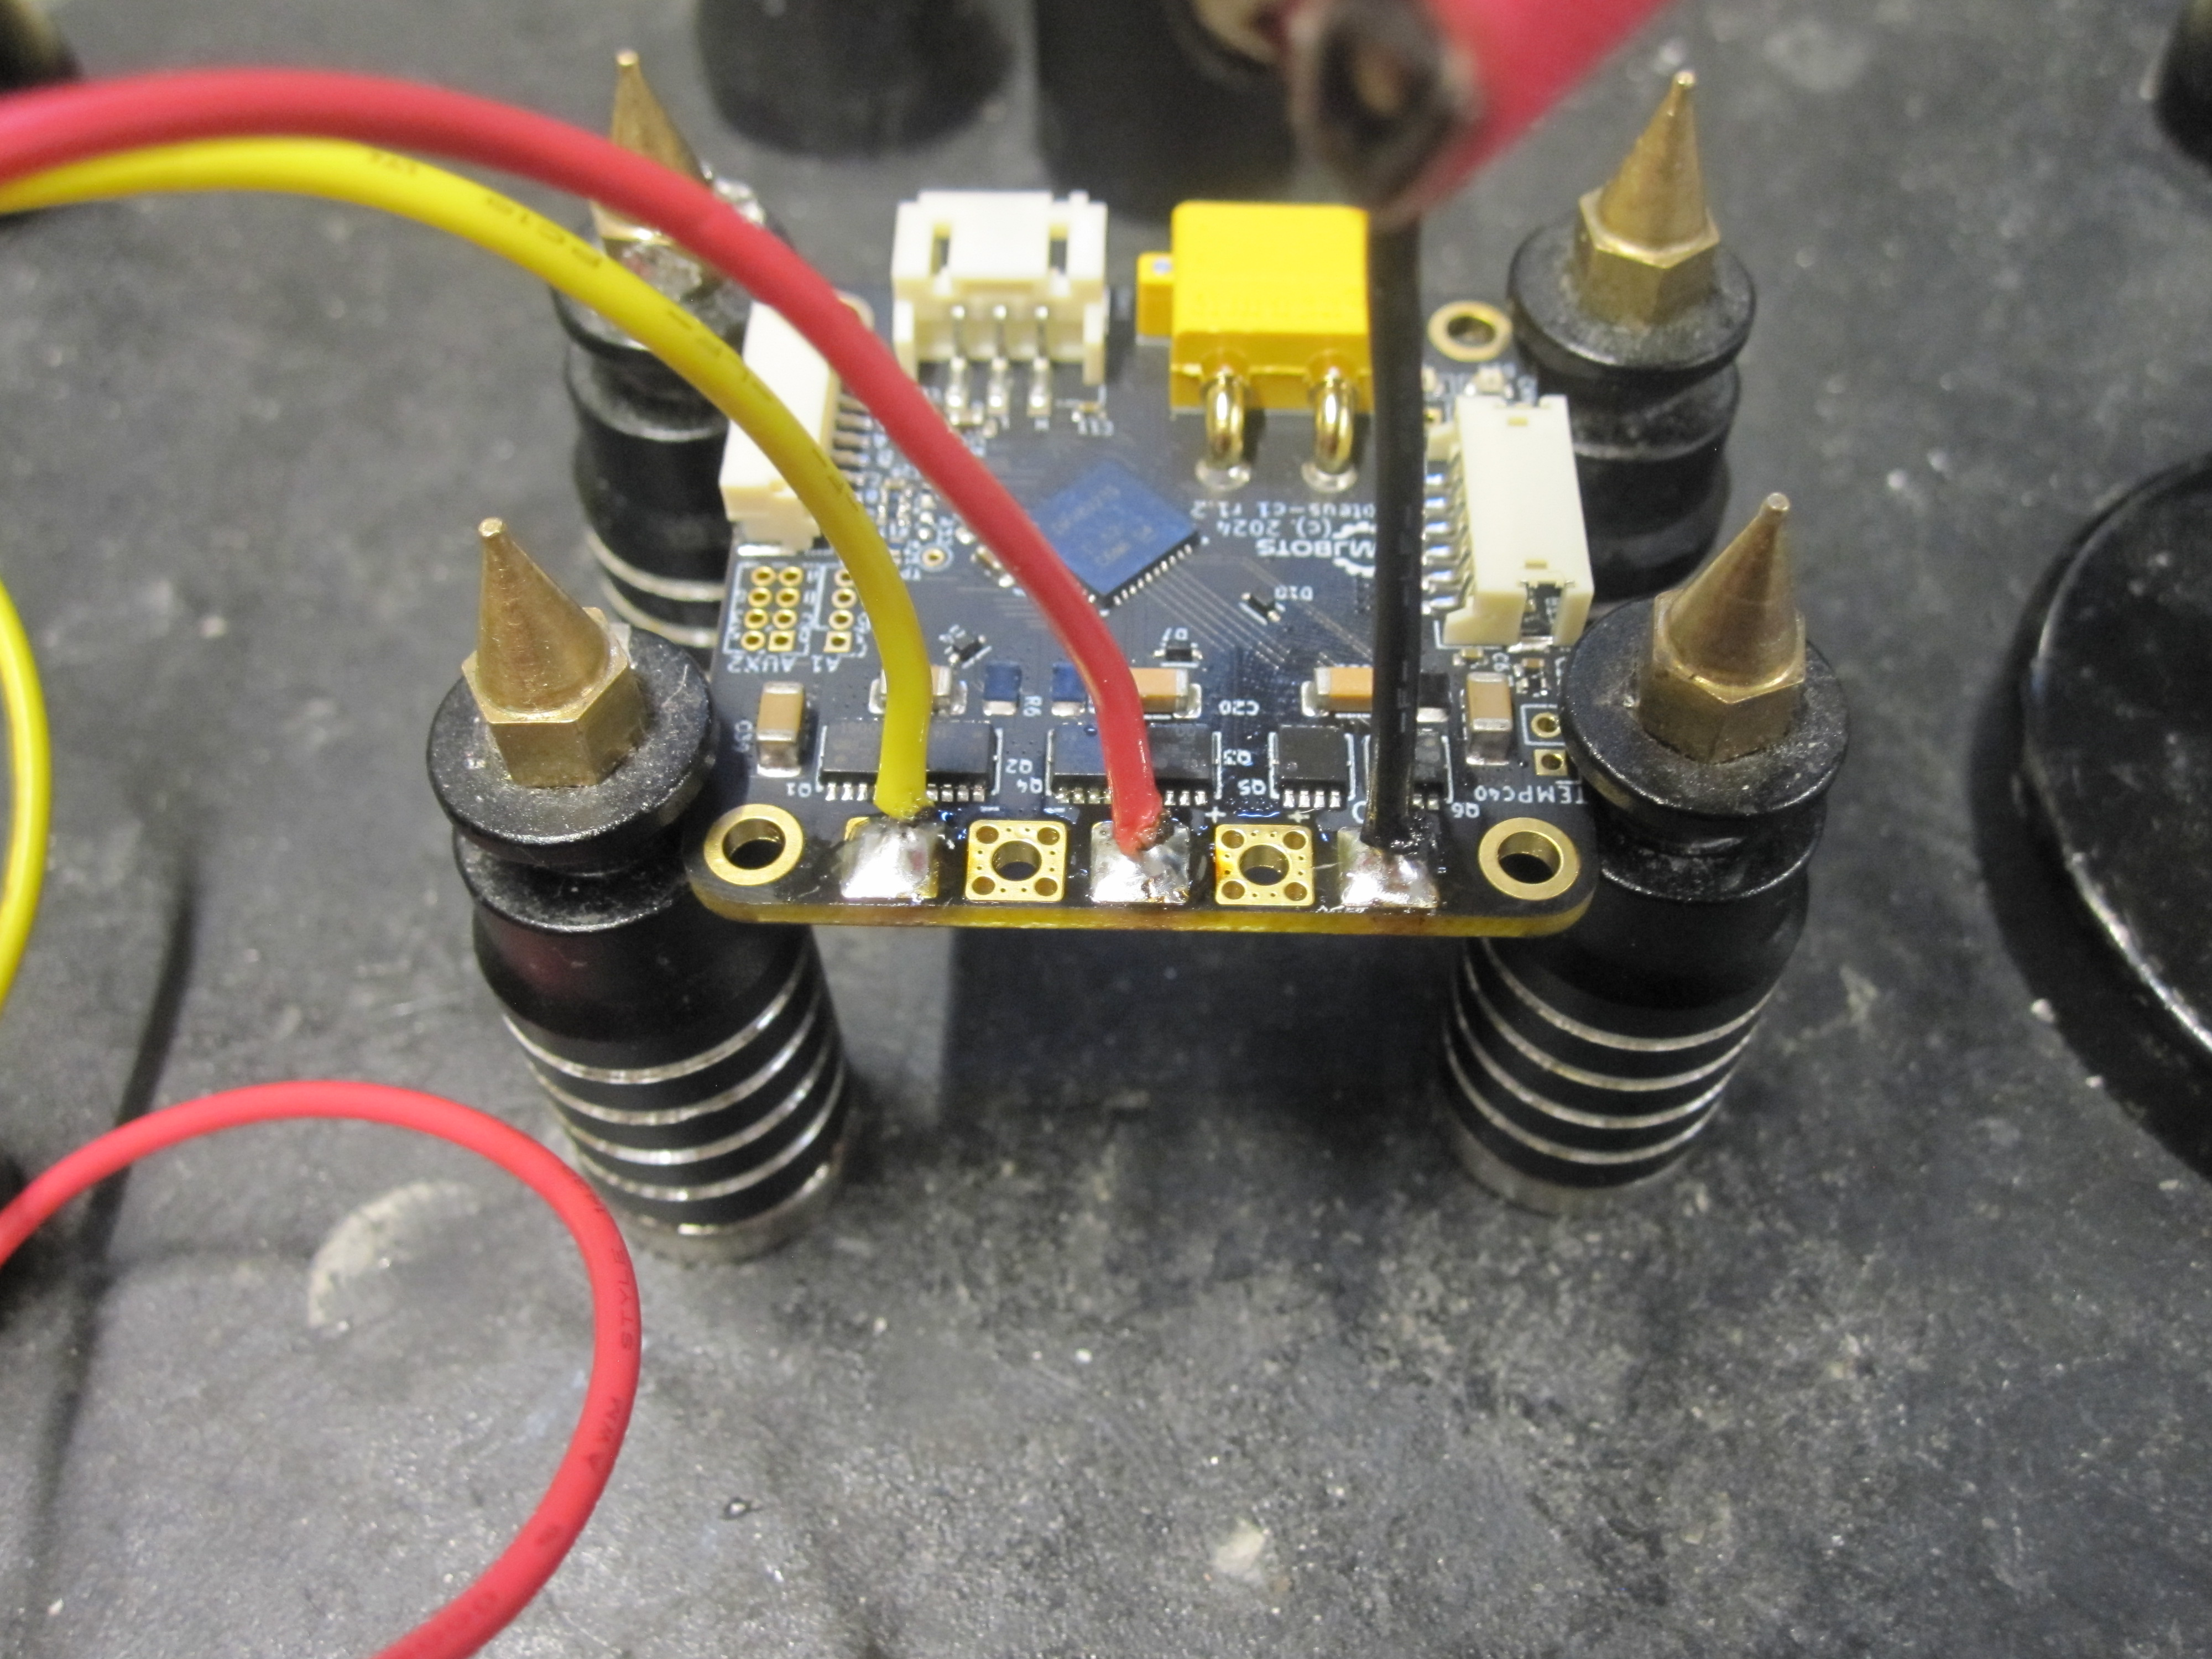
\includegraphics[width=0.7\textwidth]{fig/implementation/phase-wire-soldered.JPG}\hfill
  \caption{}
  \label{fig:soldered-moteus}
\end{figure}

The moteus boards could then be assebled on the back of the motors.


\begin{figure}[H]
  \centering
  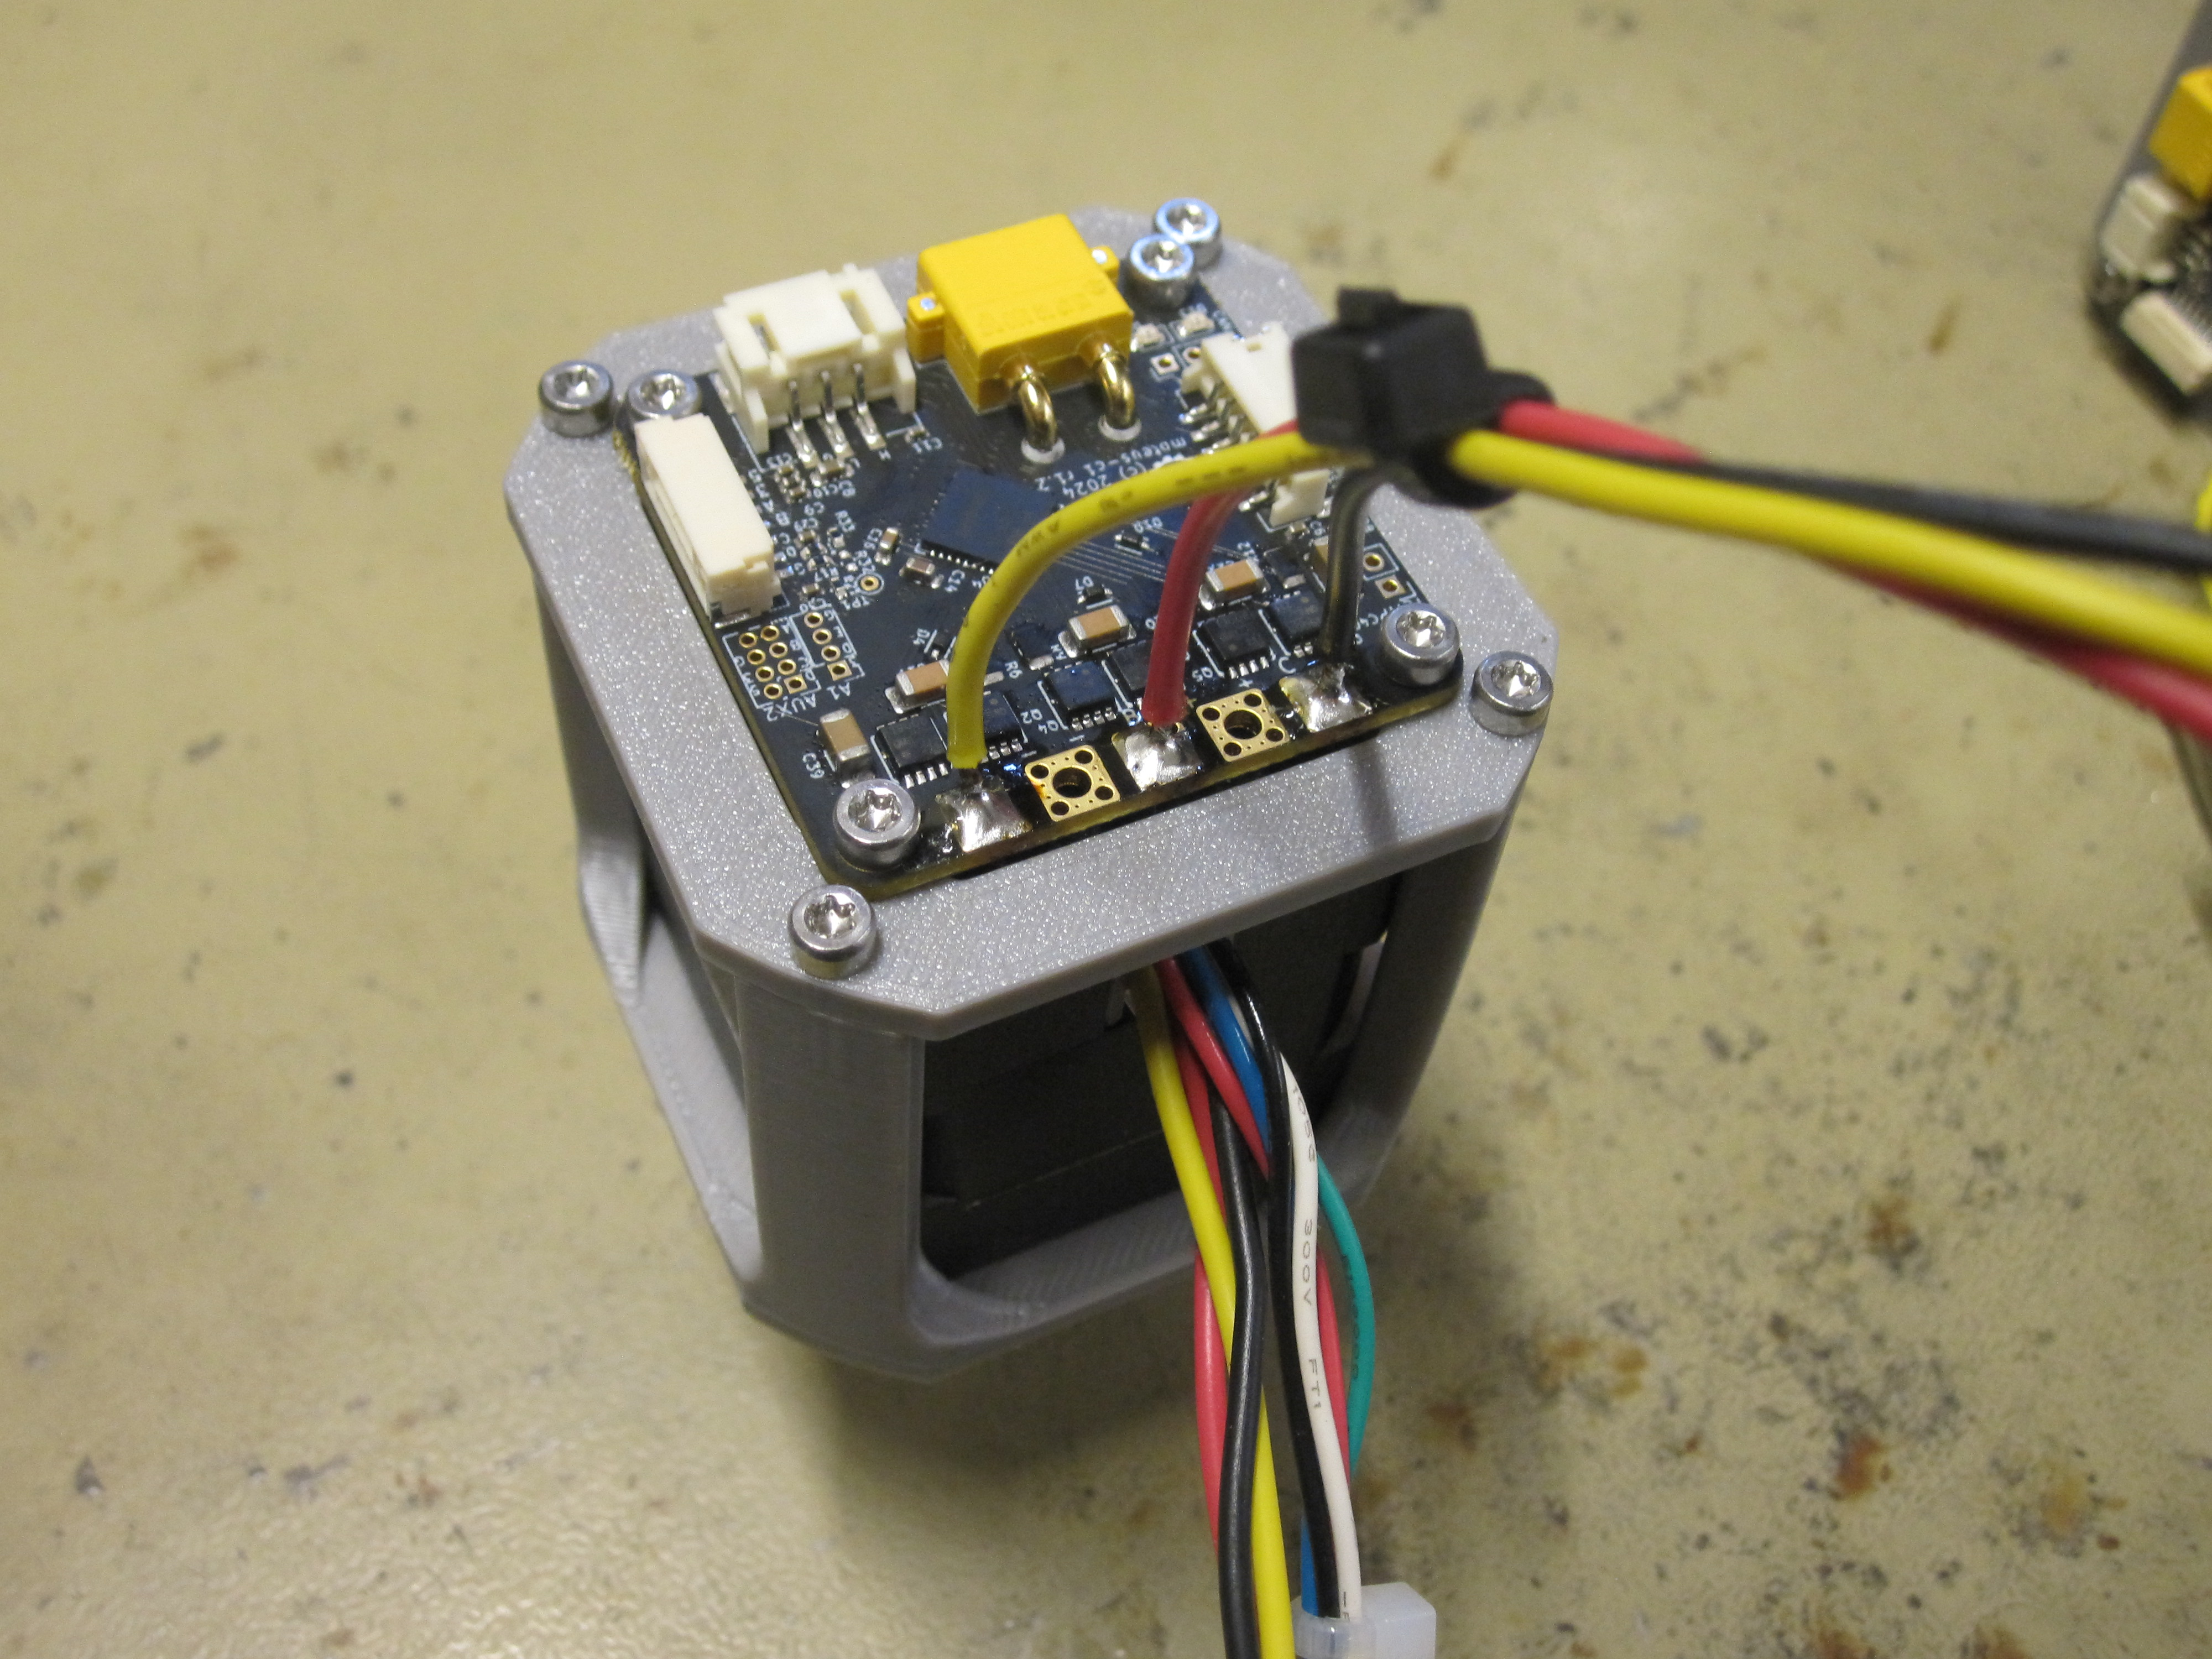
\includegraphics[width=0.7\textwidth]{fig/implementation/mounted-moteus.JPG}\hfill
  \caption{}
  \label{fig:mounted-moteus}
\end{figure}

\section{Software}



\cleardoublepage
